\begin{name}
	{\tenchude}{\tendethi}{LỚP TOÁN THẦY PHÁT}{\thoigian}
\end{name}
\Opensolutionfile{ans}[ans/ans-2-TT-1-THPTPhanChauTrinh-DaNang-23]
\setcounter{ex}{0}\setcounter{bt}{0}
\begin{ex}%[Đề thi thử môn Toán 12,THPT Phan Châu Trinh, Đà Nẵng]%[Anh Duy, 12EX-6-2223]%[2H3Y1-3]%Câu 3
	Trong KG $Oxyz$, mặt cầu $(S)\colon x^2+y^2+z^2-2x+4y-6z-5=0$ có bán kính bằng 
	\choice
	{$\sqrt{5}$}
	{$3$}
	{\True $\sqrt{19}$}
	{$9$}
	\loigiai{
	Ta có $R=\sqrt{1^2+(-2)^2+3^2+5}=\sqrt{19}$.
}
\end{ex}
\begin{ex}%[Đề thi thử môn Toán 12,THPT Phan Châu Trinh, Đà Nẵng]%[Anh Duy, 12EX-6-2223]%[2H3Y2-2]%Câu 8
	Mặt phẳng $(P)$ đi qua ba điểm $A(1; 0; 0), B(2;-1; 3), C(-1; 2; 1)$ nhận véc-tơ nào sau đây làm véc-tơ pháp tuyến?
	\choice
	{$\vec{n}_1(7; 7;-4)$}
	{$\vec{n}_2(1;-1; 3)$}
	{\True $\vec{n}_3(1; 1; 0)$}
	{$\vec{n}_4(7;-7; 0)$}
	\loigiai{
		Ta có $\overrightarrow{AB}=(1;-1;3)$, $\overrightarrow{AC}=(-2;2;1)$ nên $\left[\overrightarrow{AB}, \overrightarrow{AC}\right]=(-7;-7;0)=-7(1;1;0)$.\\
		Vậy mặt phẳng $(P)$ có một véc-tơ pháp tuyến là $\vec{n}_3(1; 1; 0)$.
	}
\end{ex}

\begin{ex}%[Đề thi thử môn Toán 12,THPT Phan Châu Trinh, Đà Nẵng]%[Anh Duy, 12EX-6-2223]%[2D3Y1-1]%Câu 9
	Khẳng định nào sau đây \textbf{sai}?
	\choice
	{$\displaystyle\int\limits \dfrac{\mathrm{\,d}x}{x^2}=\dfrac{-1}{x}+C$}
	{$\displaystyle\int\limits \mathrm{\,d}x=x+C$}
	{$\displaystyle\int\limits \dfrac{\mathrm{\,d}x}{\sin ^2x}=-\cot x+C$}
	{\True $\displaystyle\int\limits \dfrac{1}{x}\mathrm{\,d}x=\ln x+C$}
	\loigiai{
		Vì $\displaystyle\int\limits \dfrac{1}{x}\mathrm{\,d}x=\ln |x|+C$ nên phương án $\displaystyle\int\limits \dfrac{1}{x}\mathrm{\,d}x=\ln x+C$ sai.
	}
\end{ex}
\begin{ex}%[Đề thi thử môn Toán 12,THPT Phan Châu Trinh, Đà Nẵng]%[Anh Duy, 12EX-6-2223]%[2H1Y3-2]%Câu 12
	Cho một khối chóp tam giác có đáy là tam giác vuông và độ dài hai cạnh góc vuông lần lượt là $4 a$ và $3 a$, chiều cao của khối chóp là $4 a$. Thể tích (tính theo $a$) của khối chóp đó là
	\choice
	{$V=24 a^3$}
	{$V=48 a^3$}
	{$V=16 a^3$}
	{\True $V=8 a^3$}
	\loigiai{
		Thể tích khối chóp là $V=\dfrac{1}{3}Sh=\dfrac{1}{3}\cdot \dfrac{1}{2}\cdot 4a\cdot 3a\cdot 4a=8a^3$.
	}
\end{ex}
\begin{ex}%[Đề thi thử môn Toán 12,THPT Phan Châu Trinh, Đà Nẵng]%[Anh Duy, 12EX-6-2223]%[2D1Y2-2]%Câu 16
	\immini{Cho hàm số $y=a x^3+b x^2+c x+d$ có đồ thị là đường cong hình bên. Điểm cực tiểu của hàm số là
		\choice
		{$y=-2$}
		{\True $x=1$}
		{$(1;-2)$}
		{$x=0$}}
	{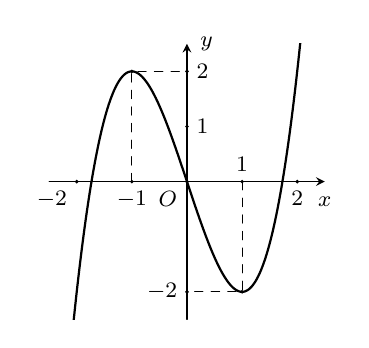
\begin{tikzpicture}[scale=.7,>=stealth, font=\footnotesize, line join=round, line cap=round]	
			\tikzset{label style/.style={font=\footnotesize}}
			\def \xmin{-2.5}\def \xmax{2.5}\def \ymin{-2.5}\def \ymax{2.5} 
			\draw[->] (\xmin,0)--(\xmax,0) node[shift=(-90:0.25)] {$x$};
			\draw[->] (0,\ymin)--(0,\ymax) node[shift=(0:0.25)] {$y$};
			\foreach \x in {-1,2}
			\fill[black] (\x,0) node[below]{$\x$}circle(1pt);
			\foreach \y in {1,2}
			\fill[black] (0,\y) node[right]{$\y$}circle(1pt);
			\fill[black] 
			(0,0)node [below left]{$O$} circle(1pt) 
			(0,-2)node [left]{$-2$} circle(1pt)
			(1,0)node [above]{$1$} circle(1pt) 
			(-2,0)node [below left]{$-2$} circle(1pt) 
			(1,-2) circle(1pt) 
			(-1,2) circle(1pt) 
			; 
			\draw[dashed] (-1,0)|-(0,2) (1,0)|-(0,-2);
			\begin{scope}
				\clip (\xmin,\ymin) rectangle (\xmax,\ymax); 
				\draw[thick,samples=200,domain=\xmin:\xmax,smooth,variable=\x] plot
				(\x,{1*((\x)^3)-3*(\x)});
			\end{scope}
	\end{tikzpicture}}
	\loigiai{Điểm cực tiểu của hàm số là $x=1$.}
\end{ex}
\begin{ex}%[Đề thi thử môn Toán 12,THPT Phan Châu Trinh, Đà Nẵng]%[Anh Duy, 12EX-6-2223]%[2D2Y3-2]%Câu 18
	Với $a$ là số thực dương tuỳ ý khác $1$, $\log _a 2 a$ bằng
	\choice
	{$1+\log _2 a$}
	{$1-\log _a 2$}
	{\True $1+\dfrac{1}{\log _2 a}$}
	{$2$}
	\loigiai{
		Ta có $\log_a 2a=\log_a 2+\log_a a=1+\log_a 2=1+\dfrac{1}{\log_2 a}$.
	}
\end{ex}

\begin{ex}%[Đề thi thử môn Toán 12,THPT Phan Châu Trinh, Đà Nẵng]%[Anh Duy, 12EX-6-2223]%[2D1Y1-2]%Câu 19
	Cho hàm số $y=f(x)$ xác định, liên tục trên $\mathbb{R}$ và có bảng biến thiên như sau:
	\begin{center}
		
\begin{tikzpicture}
			\tkzTabInit[nocadre=false,lgt=1.2,espcl=2.5,deltacl=0.6]
			{$x$/.7 ,$f'(x)$/.7,$f(x)$/2}
			{$-\infty$ , $0$ , $2$ , $+\infty$}
			\tkzTabLine{ , + , $0$ , - , $0$ , + , }
			\tkzTabVar{-/$-\infty$ , +/$2$ , -/$-3$, +/$+\infty$}
		\end{tikzpicture}
	\end{center}
	Hàm số đã cho đồng biến trên khoảng nào dưới đây?
	\choice
	{$(0; 2)$}
	{$(-\infty; 1)$}
	{\True $(3;+\infty)$}
	{$(-3;+\infty)$}
	\loigiai{Hàm số đồng biến trên khoảng $(3;+\infty)$.}
\end{ex}
\begin{ex}%[Đề thi thử môn Toán 12,THPT Phan Châu Trinh, Đà Nẵng]%[Anh Duy, 12EX-6-2223]%[2H1Y2-2]%Câu 23
	Khối bát diện đều là khối đa diện đều loại
	\choice
	{$\{4; 3\}$}
	{$\{5; 3\}$}
	{\True $\{3; 4\}$}
	{$\{3; 3\}$}
	\loigiai{Khối bát diện đều là khối đa diện đều loại $\{3; 4\}$.}
\end{ex}

\begin{ex}%[Đề thi thử môn Toán 12,THPT Phan Châu Trinh, Đà Nẵng]%[Anh Duy, 12EX-6-2223]%[2H3Y3-1]%Câu 26
	Trong KG $Oxyz$, đường thẳng $(d):\heva{&x=1+2 t\\&y=4 \\& z=-3-t}$ có một véc-tơ chỉ phương là
	\choice
	{$\vec{n}_2=(1; 4;-3)$}
	{\True $\vec{u}_4=(2; 0;-1)$}
	{$\vec{n}_1=(1; 0;-3)$}
	{$\vec{u}_3=(2; 4;-1)$}
	\loigiai{Đường thẳng $(d)$ có một véc-tơ chỉ phương là $\vec{u}_4=(2; 0;-1)$.}
\end{ex}
\begin{ex}%[Đề thi thử môn Toán 12,THPT Phan Châu Trinh, Đà Nẵng]%[Anh Duy, 12EX-6-2223]%[2H3Y1-2]%Câu 28
	Trong KG $Oxyz$, cho hai véc-tơ $\vec{u}=(1; 3;-2)$ và $\vec{v}=(2; 1; 0)$. Tích vô hướng $\vec{u}\cdot \vec{v}$ bằng
	\choice
	{$3$}
	{$\sqrt{70}$}
	{\True $5$}
	{$25$}
	\loigiai{
		Ta có $\vec{u}\cdot \vec{v}=1\cdot 2+3\cdot 1+(-2)\cdot 0=5$.
	}
\end{ex}
\begin{ex}%[Đề thi thử môn Toán 12,THPT Phan Châu Trinh, Đà Nẵng]%[Anh Duy, 12EX-6-2223]%[2D2Y2-1]%Câu 35
	Tập xác định của hàm số $y=(1-2x)^{\frac{1}{3}}$ là
	\choice
	{$\mathscr{D}=\left(\dfrac{1}{2};+\infty\right)$}
	{$\mathscr{D}=\mathbb{R}$}
	{$\mathscr{D}=\mathbb{R}\setminus \left\{\dfrac{1}{2}\right\}$}
	{\True $\mathscr{D}=\left(-\infty; \dfrac{1}{2}\right)$}
	\loigiai{
		Hàm số $y=(1-2x)^{\frac{1}{3}}$ xác định khi $1-2x>0\Leftrightarrow x<\dfrac{1}{2}$.\\
		Vậy tập xác định của hàm số là $\mathscr{D}=\left(-\infty;\dfrac{1}{2}\right)$.
	}
\end{ex}

\begin{ex}%[Đề thi thử môn Toán 12,THPT Phan Châu Trinh, Đà Nẵng]%[Anh Duy, 12EX-6-2223]%[2D2Y4-1]%Câu 36
	Hàm số nào sau đây đồng biến trên tập số thực $\mathbb{R}$?
	\choice
	{$y=5^{-x}$}
	{\True $y=\pi^x$}
	{$y=\left(\dfrac{3}{4}\right)^x$}
	{$y=\left(\dfrac{1}{2}\right)^x$}
	\loigiai{Hàm số $y=\pi^x$ có cơ số $\pi>1$ nên đồng biến trên tập số thực $\mathbb{R}$.}
\end{ex}
\begin{ex}%[Đề thi thử môn Toán 12,THPT Phan Châu Trinh, Đà Nẵng]%[Anh Duy, 12EX-6-2223]%[2H2B1-1]%Câu 2
	Một hình trụ có diện tích xung quanh bằng $S$, diện tích một mặt đáy bằng diện tích một mặt cầu có bán kính $a$. Khi đó thể tích của khối trụ tính theo $S$ và $a$ là
	\choice
	{\True $S a$}
	{$\dfrac{1}{2}S a$}
	{$\dfrac{1}{3}S a$}
	{$\dfrac{1}{4}S a$}
	\loigiai{Gọi $r$ là bán kính đáy của hình trụ và $h$ là chiều cao của hình trụ, ta có 
		\[\heva{&S=2\pi rh\\&\pi r^2=4\pi a^2}\Leftrightarrow \heva{&r=2a\\&h=\dfrac{S}{4\pi a}}\Rightarrow V=\pi r^2h=Sa.\]
	}
\end{ex}

\begin{ex}%[Đề thi thử môn Toán 12,THPT Phan Châu Trinh, Đà Nẵng]%[Anh Duy, 12EX-6-2223]%[2H3B3-6]%Câu 5
	Trong KG $Oxyz$, cho đường thẳng $d\colon  \dfrac{x}{5}=\dfrac{y+1}{-3}=\dfrac{z-4}{1}$. Trong các mặt phẳng sau đây mặt phẳng nào song song với đường thẳng $d$?
	\choice
	{$5x-3y+z+2=0$} 
	{$x+y-2z+9=0$}
	{$5x-3y+z-2=0$}
	{\True $x+3y+4z-9=0$}
	\loigiai{
	Đường thẳng $(d)$ có véc-tơ chỉ phương $\vec{u}=(5;-3;1)$.\\
	Để mặt phẳng và đường thẳng song song thì véc-tơ pháo tuyến của $(P)$ phải vuông góc với véc-tơ chỉ phương của $(d)$.\\
	Xét mặt phẳng $x+y-2z+9=0$ có $\vec{n}=(1;1;-2)$ vuông góc với $\vec{u}_d$, nhưng $(0;-1;4)\in (d)$ cũng nằm trong mặt phẳng $x+y-2z+9=0$ nên $d$ nằm trong mặt phẳng này.\\
	Xét mặt phẳng $x+3y+4z-9=0$ có $\vec{n}=(1;3;4)$ vuông góc với $\vec{u}_d$ và $(0;-1;4)\notin (P)$, do đó $(P)$ và $(d)$ song song với nhau.
}
\end{ex}

\begin{ex}%[Đề thi thử môn Toán 12,THPT Phan Châu Trinh, Đà Nẵng]%[Anh Duy, 12EX-6-2223]%[2D4B1-2]%Câu 6
	Trong mặt phẳng với hệ tọa độ $Oxy$, tập hợp điểm $M$ biểu diễn số phức $z$ thỏa mãn điều kiện $|z-i+1|=2$ là
	\choice
	{Đường tròn tâm $I(1;-1)$, bán kính $R=2$}
	{Hình tròn tâm $I(1;-1)$, bán kính $R=4$}
	{Đường tròn tâm $I(-1; 1)$, bán kính $R=4$}
	{\True Đường tròn tâm $I(-1; 1)$, bán kính $R=2$}
	\loigiai{
	Đặt $z=x+yi$ với $x,y\in \mathbb{R}$. Ta có
	\begin{eqnarray*}
	|z-i+1|=2 &\Leftrightarrow& |x+yi-i+1|=2\\
	&\Leftrightarrow& |(x+1)+(y-1)i|=2\\
	&\Leftrightarrow& (x+1)^2+(y-1)^2=4.
	\end{eqnarray*}
	Vậy tập hợp điểm $M$  biểu diễn số phức $z$ thỏa mãn điều kiện $|z-i+1|=2$ là đường tròn tâm $I(-1; 1)$, bán kính $R=2$.
}
\end{ex}


\begin{ex}%[Đề thi thử môn Toán 12,THPT Phan Châu Trinh, Đà Nẵng]%[Anh Duy, 12EX-6-2223]%[1D3B2-3]%Câu 10
	Dãy số nào sau đây là dãy tăng?
	\choice
	{$u_n=(-1)^{n+1}\sin \dfrac{\pi}{n}$}
	{$u_n=\dfrac{2 n+3}{3 n+2}$}
	{$u_n=\dfrac{1}{n+\sqrt{n+1}}$}
	{\True $u_n=(-1)^{2 n}\left(3^n+1\right)$}
	\loigiai{
	Xét dãy $u_n=(-1)^{n+1}\sin \dfrac{\pi}{n}$ có $u_1=0$, $u_2=-1<u_1$ nên $u_n$ không phải là dãy số tăng.\\
	Xét dãy $u_n=\dfrac{2 n+3}{3 n+2}$ có $u_1=1$, $u_2=\dfrac{7}{8}<u_1$ nên $u_n$ không là dãy số tăng.\\
	Xét dãy $u_n= \dfrac{1}{n+\sqrt{n+1}}$ có $u_1=-1+\sqrt{2}$, $u_2=2-\sqrt{3}<u_1$ nên $u_n$ không là dãy số tăng.\\
	Vậy $u_n=(-1)^{2 n}\left(3^n+1\right)$ là dãy số tăng.
}
\end{ex}

\begin{ex}%[Đề thi thử môn Toán 12,THPT Phan Châu Trinh, Đà Nẵng]%[Anh Duy, 12EX-6-2223]%[2D1B3-2]%Câu 11
	Tìm giá trị nhỏ nhất của hàm số $y=-x+3-\dfrac{1}{x+2}$ trên nửa khoảng $[-4;-2)$.
	\choice
	{$\min \limits_{[-4;-2)}y=6$}
	{\True $\min \limits_{[-4;-2)}y=7$}
	{$\min \limits_{[-4;-2)}y=4$}
	{$\min \limits_{[-4;-2)}y=5$}
	\loigiai{
	Tập xác định $\mathscr{D}=\mathbb{R}\setminus \{-2\}$.\\
	Ta có $y'=-1+\dfrac{1}{(x+2)^2}$.\\
	$y'=0\Leftrightarrow \hoac{&x=-1\notin [-4;-2)\\&x=-3\in [-4;-2)}$. Ta có bảng biến thiên như sau
	\begin{center}
		
\begin{tikzpicture}
			\tkzTabInit[nocadre=false,lgt=1.2,espcl=2.5,deltacl=0.6]
			{$x$/.7 ,$y'$/.7,$y$/2}
			{$-4$ , $-3$ , $-2$}
			\tkzTabLine{ , - , $0$ ,+, }
			\tkzTabVar{+/$ $ , -/$7$ , +/$ $}
		\end{tikzpicture}
	\end{center}
Dựa vào bảng biến thiên, suy ra $\min \limits_{[-4;-2)}y=7$.
}
\end{ex}

\begin{ex}%[Đề thi thử môn Toán 12,THPT Phan Châu Trinh, Đà Nẵng]%[Anh Duy, 12EX-6-2223]%[1D2B2-1]%Câu 13
	Có bao nhiêu cách xếp $4$ người Việt Nam, $5$ người Pháp và $2$ người Mỹ ngồi lên một chiếc ghế dài gồm $11$ vị trí? Biết những người cùng quốc tịch phải ngồi gần nhau.
	\choice
	{$5760$}
	{$45602$}
	{$1640$}
	{\True $34560$}
	\loigiai{
	Xếp $4$ người Việt Nam có $4!$ cách.\\
	Xếp $5$ người Pháp có $5!$ cách.\\
	Xếp $2$ người Mỹ có $2!$ cách.\\
	Coi $4$ người Việt Nam, $5$ người Pháp, $2$ người Mỹ là $3$ nhóm, sắp xếp vị trí cho họ có $3!$ cách.\\
	Theo quy tắc nhân có $4!5!2!3!=34560$ cách.
}
\end{ex}

\begin{ex}%[Đề thi thử môn Toán 12,THPT Phan Châu Trinh, Đà Nẵng]%[Anh Duy, 12EX-6-2223]%[2D1B5-3]%Câu 14
	Cho hàm số $y=f(x)=-x^3+3 x^2-4$. Có bao nhiêu giá trị của $m$ để phương trình $f(x)=m$ có ba nghiệm thực phân biệt?
	\choice
	{$4$}
	{$5$}
	{\True $3$}
	{$7$}
	\loigiai{
	Ta có $f'(x)=-3x^2+6x$.\\
	$f'(x)=0\Leftrightarrow \hoac{&x=0\\&x=2.}$\\
	Ta có bảng biến thiên như sau
	\begin{center}
		
\begin{tikzpicture}
			\tkzTabInit[nocadre=false,lgt=1.2,espcl=2.5,deltacl=0.6]
			{$x$/.7 ,$f'(x)$/.7,$f(x)$/2}
			{$-\infty$ , $0$ , $2$ , $+\infty$}
			\tkzTabLine{ , - , $0$ , +, $0$ , - , }
			\tkzTabVar{+/$+\infty$ , -/$-4$ , +/$0$, -/$-\infty$}
		\end{tikzpicture}
	\end{center}
Dựa vào bảng biến thiên ta thấy phương trình $f(x)=m$ có ba nghiệm thực phân biệt khi $-4<m<0$.\\
Suy ra $m\in \{-3;-2;-1\}$ nên có $3$ giá trị của $m$ thỏa yêu cầu bài toán.
}
\end{ex}

\begin{ex}%[Đề thi thử môn Toán 12,THPT Phan Châu Trinh, Đà Nẵng]%[Anh Duy, 12EX-6-2223]%[2D1B1-1]%Câu 15
	Cho hàm số $y=f(x)$ có đạo hàm $f'(x)=(1-x)^2(x+1) x$ với mọi $x$. Hàm số đã cho nghịch biến trên khoảng nào sau đây?
	\choice
	{$(0; 1)$}
	{\True $(-1; 0)$}
	{$(-1; 1)$}
	{$(1;+\infty)$}
	\loigiai{$f'(x)=0\Leftrightarrow \hoac{&x=1\text{ (bội $2$)}\\&x=-1\\&x=0.}$\\
	Ta có bảng xét dấu như sau
	\begin{center}
		
\begin{tikzpicture}
			\tkzTabInit[nocadre=false,lgt=1.2,espcl=2.5,deltacl=0.6]
			{$x$/.7 ,$f'(x)$/.7}
			{$-\infty$ , $-1$ , $0$ ,$1$, $+\infty$}
			\tkzTabLine{ , + , $0$ , - , $0$ , + , $0$,$+$, }
		\end{tikzpicture}
	\end{center}
Dựa vào bảng xét dấu, nhận thấy hàm số nghịch biến trên khoảng $(-1;0)$.}	
\end{ex}


\begin{ex}%[Đề thi thử môn Toán 12,THPT Phan Châu Trinh, Đà Nẵng]%[Anh Duy, 12EX-6-2223]%[2D4B1-3]%Câu 17
	Cho các mệnh đề sau:
	\begin{enumEX}{2}
	\item Mọi số thực không phải là số thuần ảo. 
	\item Mọi số thuần ảo không phải là số thực. 
	\item Phần thực của số phức là một số thực. 
	\item Phần ảo của số phức là một số thuần ảo.
	\end{enumEX}
	Số mệnh đề đúng trong các mệnh đề trên là
	\choice
	{$4$}
	{$2$}
	{$3$}
	{\True $1$}
	\loigiai{
	Mệnh đề \lq\lq  Mọi số thực không phải là số thuần ảo\rq\rq\, sai vì số thực $0$ cũng là số thuần ảo.
	Mệnh đề \lq\lq  Mọi số thuần ảo không phải là số thực\rq\rq\, sai vì $0i=0$ là số thực.\\
	Mệnh đề \lq\lq  Phần ảo của số phức là một số thuần ảo\rq\rq\, sai vì phần ảo của số phức là số thực.\\
	Vậy có $1$ mệnh đề đúng.
}
\end{ex}

\begin{ex}%[Đề thi thử môn Toán 12,THPT Phan Châu Trinh, Đà Nẵng]%[Anh Duy, 12EX-6-2223]%[2D2B6-1]%Câu 20
	Tập nghiệm của bất phương trình $\log _{\frac{1}{3}}(x+1)>0$ là
	\choice
	{$(0;+\infty)$}
	{$(-1;+\infty)$}
	{\True $(-1; 0)$}
	{$(-\infty; 0)$}
	\loigiai{
	Ta có 
	\[\log_{\frac{1}{3}}(x+1)>0\Leftrightarrow \heva{&x+1>0\\&x+1<1}\Leftrightarrow -1<x<0.\]
	Tập nghiệm của bất phương trình là $(-1;0)$.
}
\end{ex}

\begin{ex}%[Đề thi thử môn Toán 12,THPT Phan Châu Trinh, Đà Nẵng]%[Anh Duy, 12EX-6-2223]%[2H1B3-2]%Câu 21
	Cho hình chóp $S.ABCD$ có đáy $ABCD$ là hình vuông cạnh $a$, tam giác $SAB$ đều và nằm trong mặt phẳng vuông góc với đáy. Thể tích của khối chóp đã cho tính theo cạnh $a$ là
	\choice
	{\True $\dfrac{a^3 \sqrt{3}}{6}$}
	{$\dfrac{a^3 \sqrt{3}}{2}$}
	{$\dfrac{a^3}{6}$}
	{$\dfrac{a^3}{2}$}
	\loigiai{
	\immini{Gọi $H$ là trung điểm $AB$, $SH\perp (ABCD)$ và $SH=\dfrac{a\sqrt{3}}{2}$.\\
	Thể tích khối chóp là $V_{S.ABCD}=\dfrac{1}{3}\cdot SH\cdot S_{ABCD}=\dfrac{a^3\sqrt{3}}{6}$.}
{\begin{tikzpicture}[scale=0.7,>=stealth, font=\footnotesize, line join=round, line cap=round]
		\path
		(0,0) coordinate (B) 
		(40:3) coordinate (A)
		(0:5) coordinate (C)
		($(A)+(C)-(B)$) coordinate (D)
		($(A)!.5!(B)$) coordinate (H)
		($(H)+(90:4)$) coordinate (S)
		;
		
		\draw
		(S)--(B)--(C)--(D)--cycle
		(S)--(C)
		;
		\draw[dashed] (B)--(A)--(D) (A)--(S)--(H);
		\tkzMarkRightAngles(A,H,S)
		\foreach \x/\g in
		{A/-80,B/-90,C/-90,D/0,H/-90,S/90}
		\fill[black](\x) circle (2pt)
		($(\x)+(\g:5mm)$) node{$\x$};
\end{tikzpicture}
}
}
\end{ex}

\begin{ex}%[Đề thi thử môn Toán 12,THPT Phan Châu Trinh, Đà Nẵng]%[Anh Duy, 12EX-6-2223]%[2D2B5-2]%Câu 22
	Số nghiệm thực của phương trình $3^{x^2-2}=81$ là
	\choice
	{\True $2$}
	{$1$}
	{$0$}
	{$3$}
	\loigiai{Ta có 
	\begin{eqnarray*}
	3^{x^2-2}=81 &\Leftrightarrow& 3^{x^2-2}=3^4\\
	&\Leftrightarrow& x^2-2=4\\
	&\Leftrightarrow& x^2=6\\
	&\Leftrightarrow& x=\pm \sqrt{6}.
	\end{eqnarray*}
	Vậy phương trình có 2 nghiệm thực.
}
\end{ex}

\begin{ex}%[Đề thi thử môn Toán 12,THPT Phan Châu Trinh, Đà Nẵng]%[Anh Duy, 12EX-6-2223]%[2D2B3-2]%Câu 24
	Cho $a, b$ là các số thực dương tùy ý thỏa mãn $3 \log _2 a-\log _4 b=1$. Mệnh đề nào sau đây là mệnh đề đúng?
	\choice
	{\True $a^3=2 \sqrt{b}$}
	{$a^3 b^2=2$}
	{$a^3=2 b^2$}
	{$a^3 \sqrt{b}=2$}
	\loigiai{
	Ta có 
	\allowdisplaybreaks
	\begin{eqnarray*}
	3 \log _2 a-\log _4 b=1 &\Leftrightarrow& \log_2 a^3=\log_2 2+\dfrac{1}{2}\log_2 b\\
	&\Leftrightarrow& \log_2 a^3=\log_2 2b^{\frac{1}{2}}\\
	&\Leftrightarrow & a^3=2\sqrt{b}.
	\end{eqnarray*}
}
\end{ex}

\begin{ex}%[Đề thi thử môn Toán 12,THPT Phan Châu Trinh, Đà Nẵng]%[Anh Duy, 12EX-6-2223]%[2H2B1-1]%Câu 25
	Trong không gian, cho tam giác $ABC$ vuông tại $A, AB=a \sqrt{3}$ và $BC=2 a$. Khi quay tam giác $ABC$ quanh cạnh $AB$ thì đường gấp khúc $BCA$ tạo thành một hình nón tròn xoay. Thể tích của khối nón tròn xoay tạo nên bởi hình nón tròn xoay nói trên là
	\choice
	{$\pi a^3 \sqrt{3}$}
	{$\dfrac{2 \pi a^3}{3}$}
	{\True $\dfrac{\pi a^3 \sqrt{3}}{3}$}
	{$2 \pi a^3$}
	\loigiai{
	\immini{Hình nón tạo thành có chiều cao $AB=a\sqrt{3}$ và đường sinh $BC=2a$ nên nó có bán kính đáy là 
	\[AC=\sqrt{BC^2-AB^2}=\sqrt{(2a)^2-\left(a\sqrt{3}\right)^2}=a.\]
	Thể tích khối nón tạo thành là 
	$$V=\dfrac{1}{3}\pi AC^2\cdot AB=\dfrac{1}{3}\pi a^2a\sqrt{3}=\dfrac{\pi a^3\sqrt{3}}{3}.$$}
	{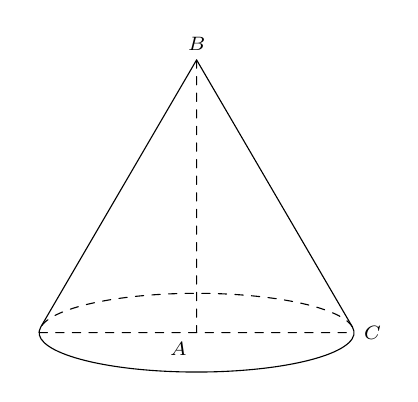
\begin{tikzpicture}[line
			join=round,line
			cap=round,font=\scriptsize]
			\def\a{2}
			\def\b{.5}
			\pgfmathsetmacro\h{\a*sqrt(3)} 
			\pgfmathsetmacro\g{asin(\b/\h)}
			\pgfmathsetmacro\xo{\a*cos(\g)}
			\pgfmathsetmacro\yo{\b*sin(\g)}
			\draw[dashed]
			(\xo,\yo) arc (\g:180-\g:{\a} and
			{\b})
			(180:\a) --(0:\a)
			node[right]{$C$} (90:\h) node[above]{$B$}--(0:0)
			node[below left]{$A$}
			;
			\draw (90:\h)--(-\xo,\yo) arc
			(180-\g:360+\g:{\a} and
			{\b})--cycle;
	\end{tikzpicture}}
}
\end{ex}

\begin{ex}%[Đề thi thử môn Toán 12,THPT Phan Châu Trinh, Đà Nẵng]%[Anh Duy, 12EX-6-2223]%[2H3B2-3]%Câu 27
	Trong KG $Oxyz$, cho hai điểm $A(-1; 0; 1), B(2; 1; 1)$ và mặt phẳng \break $(\beta)\colon x-y-2z=0$. Mặt phẳng $(\alpha)$ đi qua $A, B$ và vuông góc với $(\beta)$ có phương trình là
	\choice
	{$(\alpha)\colon x+3y+2z+1=0$}
	{$(\alpha)\colon x+3y+2z-1=0$}
	{$(\alpha)\colon x-3y+2z+1=0$}
	{\True $(\alpha)\colon x-3y+2z-1=0$}
	\loigiai{
	Ta có $\overrightarrow{AB}=(3;1;0)$, véc-tơ pháp tuyến của mặt phẳng $(\beta)$ là $\overrightarrow{n}_{\beta}=(1;-1;-2)$.\\
	Suy ra $\left[\overrightarrow{AB},\overrightarrow{n}_{\beta}\right]=(-2;6;-4)$, khi đó mặt phẳng $(\alpha)$ qua $A(-1;0;1)$ và có véc-tơ pháp tuyến là $(1;-3;2)$ có phương trình 
	\[(\alpha)\colon x-3y+2z-1=0.\]
}
\end{ex}

\begin{ex}%[Đề thi thử môn Toán 12,THPT Phan Châu Trinh, Đà Nẵng]%[Anh Duy, 12EX-6-2223]%[1D3B3-5]%Câu 29
	Một cấp số cộng có $11$ số hạng. Số hạng chính giữa bằng $15$. Tổng các số hạng đó bằng
	\choice
	{$115$}
	{\True $165$}
	{$195$}
	{$120$}
	\loigiai{
	Ta có $u_6=15\Rightarrow u_1+5d=15$.\\
	Khi đó 
	\[S_{11}=\dfrac{11(2u_1+10d)}{2}=11(u_1+5d)=11\cdot 15=165.\]
}
\end{ex}

\begin{ex}%[Đề thi thử môn Toán 12,THPT Phan Châu Trinh, Đà Nẵng]%[Anh Duy, 12EX-6-2223]%[2D3B2-1]%Câu 30
	Nếu $\displaystyle\int\limits_1^2 f(x) \mathrm{\,d}x=2$ thì $I=\displaystyle\int\limits_1^2[3 f(x)-2] \mathrm{\,d}x$ bằng
	\choice
	{\True $I=4$}
	{$I=3$}
	{$I=2$}
	{$I=1$}
	\loigiai{
	Ta có $I=\displaystyle\int_{1}^2\limits \left[3f(x)-2\right]\mathrm{\,d}x=3\displaystyle\int_{1}^2\limits f(x) \mathrm{\,d}x-\displaystyle\int_{1}^2\limits 2 \mathrm{\,d}x=3\cdot 2-2=4$.
}
\end{ex}
\begin{ex}%[Đề thi thử môn Toán 12,THPT Phan Châu Trinh, Đà Nẵng]%[Anh Duy, 12EX-6-2223]%[2D3B2-2]%Câu 32
	Giá trị $\displaystyle\int\limits_0^{\frac{\pi}{2}}(1-\cos x)^n \sin x \mathrm{\,d}x$ bằng
	\choice
	{$\dfrac{1}{n-1}$}
	{$\dfrac{1}{2 n}$}
	{$-\dfrac{1}{n+1}$}
	{\True $\dfrac{1}{n+1}$}
	\loigiai{
	Ta có 
	\begin{eqnarray*}
	\displaystyle\int\limits_0^{\frac{\pi}{2}}(1-\cos x)^n \sin x \mathrm{\,d}x &=& \displaystyle\int\limits_0^{\frac{\pi}{2}}(1-\cos x)^n\mathrm{\,d}(1-\cos x)\\
	&=& \dfrac{1}{n+1}(1-\cos x)^{n+1}\big|_0^{\frac{\pi}{2}}=\dfrac{1}{n+1}.	
	\end{eqnarray*}
}
\end{ex}

\begin{ex}%[Đề thi thử môn Toán 12,THPT Phan Châu Trinh, Đà Nẵng]%[Anh Duy, 12EX-6-2223]%[2H3B3-2]%Câu 33
	Trong KG $Oxyz$, cho điểm $M(-1; 2; 3)$ và mặt phẳng $(P)\colon  x-2y+z-4=0$. Đường thẳng đi qua $M$ và vuông góc với $(P)$ có phương trình là
	\choice
	{$\heva{&x=1+t \\ &y=-2-2 t \\&z=-3+t}$}
	{\True $\heva{&x=t \\& y=-2 t \\&z=4+t}$}
	{$\heva{&x=1-t \\ &y=-2+2 t \\&z=1+3 t}$}
	{$\heva{&x=-1+t \\& y=2+2 t \\&z=3+t}$}
	\loigiai{Gọi $d$ là đường thẳng qua $M$ và vuông góc với $(P)$.\\
	Suy ra đường thẳng $d$ có véc-tơ chỉ phương $\vec{u}=(1;-2;1)$ và có PTTS là $\heva{&x=-1+t\\&y=2-2t\\&z=3+t.}$\\
	Lấy $N\in d$, suy ra $N(0;0;4)$.\\
	Vậy PTTS của $d$ là $\heva{&x=t \\& y=-2 t \\&z=4+t}$.
}
\end{ex}

\begin{ex}%[Đề thi thử môn Toán 12,THPT Phan Châu Trinh, Đà Nẵng]%[Anh Duy, 12EX-6-2223]%[2D3B3-3]%Câu 34
	Cho hình phẳng $(H)$ giới hạn bởi đồ thị hàm số $y=e^x$, các đường thẳng $x=0, x=\ln 3$ và trục hoành. Thể tích khối tròn xoay sinh bởi $(H)$ khi quay quanh trục hoành là
	\choice
	{$2 \pi$}
	{\True $4 \pi$}
	{$4$}
	{$\pi$}
	\loigiai{
	Ta có $V=\pi \displaystyle\int_{0}^{\ln 3}\limits e^{2x} \mathrm{\,d}x	=\pi \dfrac{1}{2} e^{2x}\big|_0^{\ln 3}=4\pi$.
}
\end{ex}


\begin{ex}%[Đề thi thử môn Toán 12,THPT Phan Châu Trinh, Đà Nẵng]%[Anh Duy, 12EX-6-2223]%[2D1B5-1]%Câu 37
	\immini{Đồ thị của hàm số nào sau đây có dạng như đường cong hình bên?
	\choice
	{$y=\dfrac{x-2}{x+1}$}
	{$y=x^4+2x^2-3$}
	{$y=x^4-3 x^2-3$}
	{\True $y=x^4-2x^2-3$}}
	{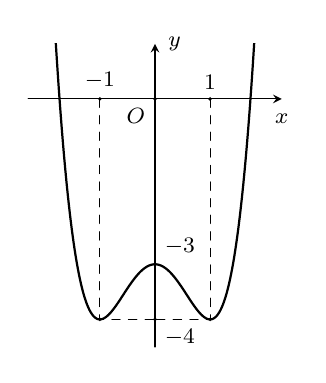
\begin{tikzpicture}[scale=.7,>=stealth, font=\footnotesize, line join=round, line cap=round]	
			\tikzset{label style/.style={font=\footnotesize}}
			\def \xmin{-2.3}\def \xmax{2.3}\def \ymin{-4.5}\def \ymax{1} 
			\draw[->] (\xmin,0)--(\xmax,0) node[shift=(-90:0.25)] {$x$};
			\draw[->] (0,\ymin)--(0,\ymax) node[shift=(0:0.25)] {$y$};
			\foreach \x in {-1,1}
			\fill[black] (\x,0) node[above]{$\x$}circle(1pt);
			\fill[black] 
			(0,0)node [below left]{$O$} circle(1pt) 
			(0,-3)node [above right]{$-3$} circle(1pt) 
			(0,-4)node [below right]{$-4$} circle(1pt) 
			(-1,-4) circle(1pt) 
			(1,-4) circle(1pt) 
			; 
			\draw[dashed] (-1,0)|-(0,-4) (1,0)|-(0,-4);
			\begin{scope}
				\clip (\xmin,\ymin) rectangle (\xmax,\ymax); 
				\draw[thick,samples=200,domain=\xmin:\xmax,smooth,variable=\x] plot
				(\x,{1*((\x)^4)-2*((\x)^2)-3});
			\end{scope}
	\end{tikzpicture}}
	\loigiai{Đường cong đã cho có dạng của đồ thị hàm bậc bốn trùng phương nên loại hàm số $y=\dfrac{x-2}{x+1}$.\\
	Hàm số có ba điểm cực trị $x=-1$, $x=0$, $x=1$ nên loại các hàm số $y=x^4+2x^2-3$, $y=x^4-3 x^2-3$.\\
	Vậy đường cong trên hình là của hàm số $y=x^4-2x^2-3$.}
\end{ex}

\begin{ex}%[Đề thi thử môn Toán 12,THPT Phan Châu Trinh, Đà Nẵng]%[Anh Duy, 12EX-6-2223]%[2D1B4-1]%Câu 38
	Số đường tiệm cận đứng và ngang của đồ thị hàm số $y=\dfrac{-2x+1}{\sqrt{4x^2-x+5}}$ là
	\choice
	{\True $2$}
	{$1$}
	{$3$}
	{$0$}
	\loigiai{
	Vì $4x^2-x+5>0,\forall x\in \mathbb{R}$ nên hàm số có tập xác định là $\mathbb{R}$.\\
	Hàm số đã cho liên tục trên $\mathbb{R}$ nên đồ thị không có tiệm cận đứng.\\
	Ta có 
	\begin{itemize}
	\item $\lim \limits_{x\to +\infty} y=\lim \limits_{x\to +\infty} \dfrac{-2x+1}{\sqrt{4x^2-x+5}}=-1$.
	\item $\lim \limits_{x\to -\infty} y=\lim \limits_{x\to -\infty} \dfrac{-2x+1}{\sqrt{4x^2-x+5}}=1$.
	\end{itemize}
	Vậy đồ thị hàm số hai đường tiệm cận ngang.
}
\end{ex}

\begin{ex}%[Đề thi thử môn Toán 12,THPT Phan Châu Trinh, Đà Nẵng]%[Anh Duy, 12EX-6-2223]%[2D1B2-1]%Câu 39
	Đồ thị của hàm số $y=3x^4-4 x^3-6x^2+12x+1$ có điểm cực tiểu là $M\left(x_1; y_1\right)$. Tính $S=x_1+y_1$.
	\choice
	{\True $S=-11$}
	{$S=6$}
	{$S=-5$}
	{$S=5$}
	\loigiai{
	Ta có $y'=12x^3-12x^2-12x+12$.\\
	$y'=0\Leftrightarrow \hoac{&x=-1\\&x=1\text{ (bội 2)}.}$\\
	Ta có bảng xét dấu như sau
	\begin{center}
		
\begin{tikzpicture}
			\tkzTabInit[nocadre=false,lgt=1.2,espcl=2.5,deltacl=0.6]
			{$x$/.7 ,$f'(x)$/.7}
			{$-\infty$ , $-1$ , $1$ , $+\infty$}
			\tkzTabLine{ , - , $0$ , + , $0$ , + , }
		\end{tikzpicture}
	\end{center}
Đồ thị hàm số $y=3x^4-4 x^3-6x^2+12x+1$ có điểm cực tiểu là $(-1;-10)$.\\
Khi đó $S=-1-10=-11$.
}
\end{ex}

\begin{ex}%[Đề thi thử môn Toán 12,THPT Phan Châu Trinh, Đà Nẵng]%[Anh Duy, 12EX-6-2223]%[2D4B2-2]%Câu 40
	Môđun của số phức $z=5+2 i-(1+i)^2$ là
	\choice
	{\True $5$}
	{$3$}
	{$4$}
	{$2$}
	\loigiai{Ta có $z=5+2i-(1+i)^2=5$.\\
	Suy ra $|z|=5$.}
\end{ex}

\begin{ex}%[Đề thi thử môn Toán 12,THPT Phan Châu Trinh, Đà Nẵng]%[Anh Duy, 12EX-6-2223]%[2D4B2-4]%Câu 41
	Trên mặt phẳng tọa độ $Oxy$ gọi $A$ là điểm biểu diễn cho số phức $z$ và $B$ là điểm biểu diễn cho số phức $-\overline{z}$. Chọn mệnh đề đúng trong các mệnh đề sau:
	\choice
	{Hai điểm $A$ và $B$ đối xứng với nhau qua đường thẳng $y=-x$}
	{\True Hai điểm $A$ và $B$ đối xứng với nhau qua trục tung}
	{Hai điểm $A$ và $B$ đối xứng với nhau qua trục hoành}
	{Hai điểm $A$ và $B$ đối xứng với nhau qua đường thẳng $y=x$}
	\loigiai{
	Gọi $z=a+b i,(a, b \in \mathbb{R}) \Rightarrow-\overline{z}=-a+bi$.\\
	Suy ra $A(a; b), B(-a; b)$ đối xứng với nhau qua trục tung.
}
\end{ex}

\begin{ex}%[Đề thi thử môn Toán 12,THPT Phan Châu Trinh, Đà Nẵng]%[Anh Duy, 12EX-6-2223]%[2H1B3-2]%Câu 42
	Hình lập phương có đường chéo của một mặt bên bằng $4 \mathrm{~cm}$. Thể tích khối lập phương đó là
	\choice
	{$8 \mathrm{~cm}^3$}
	{$2 \sqrt{2}\mathrm{~cm}^3$}
	{\True $16 \sqrt{2}\mathrm{~cm}^3$}
	{$8 \sqrt{2}\mathrm{~cm}^3$}
	\loigiai{
	Độ dài cạnh hình lập phương là $\dfrac{4}{\sqrt{2}}=2 \sqrt{2}\mathrm{~cm}$.\\
	Vậy thể tích khối lập phương đó là $V=\left(2 \sqrt{2}\right)^3=16 \sqrt{2}\mathrm{~cm}^3$.
}
\end{ex}
\begin{ex}%[Đề thi thử môn Toán 12,THPT Phan Châu Trinh, Đà Nẵng]%[Anh Duy, 12EX-6-2223]%[2D3K3-2]%Câu 4
	\immini{Một công ty quảng cáo muốn làm một bức tranh trang trí như phần $MNEIF$ được tô đậm trong hình vẽ bên, ở chính giữa của một bức tường hình chữ nhật $ABCD$ có $BC=6$ m, $CD=12$ m.
		Biết $MN=4$ m; cung $EIF$ có hình parabol với đỉnh $I$ là trung điểm của cạnh $AB$ và đi qua hai điểm $C$, $D$. Kinh phí làm bức tranh là $1\,200\,000$ đồng $/\mathrm{m}^2$. Hỏi công ty đó cần bao nhiêu tiền để làm bức tranh?
		\choice
		{$34\,266\,666$ đồng}
		{$13\,866\,666$ đồng}
		{$14\,933\,333$ đồng}
		{\True $27\,733\,333$ đồng}}
	{\begin{tikzpicture}[scale=.5,>=stealth, font=\footnotesize, line join=round, line cap=round]	
			%	\tikzset{label style/.style={font=\footnotesize}}
			\def \xmin{-6}\def \xmax{6}\def \ymin{0}\def \ymax{7} 
			\path 
			(0,0) coordinate (O)
			(-2,0) coordinate (M)
			(2,0) coordinate (N)
			(-6,0) coordinate (D)
			(6,0) coordinate (C)
			($(D)+(90:6)$) coordinate (A)
			($(C)+(90:6)$) coordinate (B)
			($(A)!.5!(B)$) coordinate (I)
			(2,16/3) coordinate (E)
			(-2,16/3) coordinate (F)
			;
			\draw (A)--(B)--(C)--(D)--cycle
			(M)--(F) (E)--(N)
			;
			\begin{scope}
				\clip (\xmin,\ymin) rectangle (\xmax,\ymax); 
				\draw[dashed,thick,samples=200,domain=\xmin:\xmax,smooth,variable=\x] plot
				(\x,{-1/6*((\x)^2)+6});
			\end{scope}
			\fill[pattern=crosshatch dots,smooth]
			plot[domain=-2:2] (\x,{0})
			-- plot[domain=2:-2] (\x,{-1/6*((\x)^2)+6})
			-- cycle;
			\draw[<->] ([yshift=-0.15cm]M) -- ([yshift=-0.15cm]N) node[midway, below]{4 m};
			\draw[<->] ([yshift=+1cm]A) -- ([yshift=+1cm]B) node[midway, above]{12 m};
			\draw[<->] ([xshift=+0.15cm]B) -- ([xshift=+0.15cm]C) node[midway, right]{6 m};
			\foreach \x/\g in
			{A/180,B/0,C/-90,D/-90,M/-90,N/-90,I/90,E/0,F/180}
			\fill[black](\x) circle (2pt)
			($(\x)+(\g:5mm)$) node{$\x$};
	\end{tikzpicture}}
	\loigiai{
		\begin{center}
			\begin{tikzpicture}[scale=.5,>=stealth, font=\footnotesize, line join=round, line cap=round]	
				%	\tikzset{label style/.style={font=\footnotesize}}
				\def \xmin{-6}\def \xmax{6}\def \ymin{0}\def \ymax{7} 
				\draw[->] (\xmin-1,0)--(\xmax+1,0) node[shift=(-90:0.25)] {$x$};
				\draw[->] (0,\ymin-1)--(0,\ymax+1) node[shift=(0:0.25)] {$y$};
				\path 
				(0,0) coordinate (O)
				(-2,0) coordinate (M)
				(2,0) coordinate (N)
				(-6,0) coordinate (D)
				(6,0) coordinate (C)
				($(D)+(90:6)$) coordinate (A)
				($(C)+(90:6)$) coordinate (B)
				($(A)!.5!(B)$) coordinate (I)
				(2,16/3) coordinate (E)
				(-2,16/3) coordinate (F)
				;
				\draw (A)--(B)--(C)--(D)--cycle
				(M)--(F) (E)--(N)
				;
				\begin{scope}
					\clip (\xmin,\ymin) rectangle (\xmax,\ymax); 
					\draw[dashed,thick,samples=200,domain=\xmin:\xmax,smooth,variable=\x] plot
					(\x,{-1/6*((\x)^2)+6});
				\end{scope}
				\fill[pattern=crosshatch dots,smooth]
				plot[domain=-2:2] (\x,{0})
				-- plot[domain=2:-2] (\x,{-1/6*((\x)^2)+6})
				-- cycle;
%				\draw[<->] ([yshift=-0.15cm]M) -- ([yshift=-0.15cm]N) node[midway, below]{4 m};
%				\draw[<->] ([yshift=+1cm]A) -- ([yshift=+1cm]B) node[midway, above]{12 m};
%				\draw[<->] ([xshift=+0.15cm]B) -- ([xshift=+0.15cm]C) node[midway, right]{6 m};
				\foreach \x/\g in
				{A/180,B/0,C/-90,D/-90,M/-90,N/-90,I/60,E/0,F/180,O/-130}
				\fill[black](\x) circle (2pt)
				($(\x)+(\g:5mm)$) node{$\x$};
			\end{tikzpicture}
		\end{center}
		Chọn hệ trục tọa độ $Oxy$ với $O$ là trung điểm cạnh $MN$.\\
		Suy ra $M(-2;0)$, $N(2;0)$.\\
		Phương trình parabol đỉnh $I(0;6)$ và đi qua hai điểm $D(-6;0)$, $C(6;0)$ là $(P)\colon y=-\dfrac{1}{6}x^2+6$.\\
		Diện tích giới hạn bởi $(P)\colon y=-\dfrac{1}{6}x^2+6$; $y=0$; $x=-2$; $x=2$ là 
		\[\displaystyle\int_{-2}^2\limits \left| -\dfrac{1}{6}x^2+6\right|  \mathrm{\,d}x=\dfrac{208}{9}\text{ m}^2.\]
		Vậy công ty đó cần $\dfrac{208}{9}\cdot 1\,200\,000=27\,733\,333$ đồng để làm bức tranh.
	}
\end{ex}
\begin{ex}%[Đề thi thử môn Toán 12,THPT Phan Châu Trinh, Đà Nẵng]%[Anh Duy, 12EX-6-2223]%[2D1K2-4]%Câu 7
	Có bao nhiêu giá trị nguyên của tham số $m$ để hàm số $y=x^3-3(m+1) x^2+9x-m$ có hai điểm cực trị tại $x_1, x_2$ thỏa $\left|x_1-x_2\right| \leq 2$?
	\choice
	{$4$}
	{$3$}
	{\True $2$}
	{$5$}
	\loigiai{
		Ta có $y=x^3-3(m+1) x^2+9x-m\Rightarrow y'=3x^2-6(m+1)x+9$.\\
		Hàm số có hai điểm cực trị khi và chỉ khi 
		\allowdisplaybreaks
		\begin{eqnarray*}
			\Delta'=9(m+1)^2-27>0&\Leftrightarrow& 9m^2+18m-18>0\\
			&\Leftrightarrow& \hoac{&m<-1-\sqrt{3}\\&m>-1+\sqrt{3}.}
		\end{eqnarray*}
		Theo hệ thức Vi-ét, ta có $\heva{&x_1+x_2=2(m+1)\\&x_1x_2=3}$.
		Khi đó ta có 
		\allowdisplaybreaks
		\begin{eqnarray*}
			\left|x_1-x_2\right| \leq 2 &\Leftrightarrow& (x_1-x_2)^2\le 4 \\
			&\Leftrightarrow& (x_1+x_2)^2-4x_1x_2\le 4\\
			&\Leftrightarrow& 4(m+1)^2-4\cdot 3\le 4\\
			&\Leftrightarrow& m^2+2m-3\le 0\\
			&\Leftrightarrow& -3\le m\le 1.
		\end{eqnarray*}
		Kết hợp điều kiện ta được $\hoac{&-3\le m< -1-\sqrt{3}\\&-1+\sqrt{3}<m\le 1.}$\\
		Vậy có $2$ giá trị nguyên của tham số $m$ là $-3;1$.
	}
\end{ex}
\begin{ex}%[Đề thi thử môn Toán 12,THPT Phan Châu Trinh, Đà Nẵng]%[Anh Duy, 12EX-6-2223]%[2H1K3-2]%Câu 1
	Cho lăng trụ $ABC.A'B'C'$. Đường thẳng đi qua trọng tâm của tam giác $ABC$ và song song với $BC$ cắt các cạnh $AB, A C$ lần lượt tại $M, N$. Mặt phẳng $\left(A'M N\right)$ chia khối lăng trụ thành hai phần. Tỉ số thể tích của phần bé và phần lớn là
	\choice
	{\True $\dfrac{4}{23}$}
	{$\dfrac{2}{3}$}
	{$\dfrac{4}{9}$}
	{$\dfrac{4}{27}$}
	\loigiai{
		\immini{Gọi $G$ là trọng tâm của tam giác $ABC$.\\ Gọi $E$ là trung điểm của $BC \Rightarrow \dfrac{AG}{AE}=\dfrac{2}{3}$.\\
			Đường thẳng $d$ đi qua $G$ và song song $BC$, cắt các cạnh $AB, A C$ lần lượt tại $M, N$. Khi đó $$\dfrac{AM}{AB}=\dfrac{AN}{A C}=\dfrac{AG}{A E}=\dfrac{2}{3}\Rightarrow \heva{&AM=\dfrac{2}{3}AB \\&AN=\dfrac{2}{3}AC}\Rightarrow S_{\triangle AMN}=\dfrac{4}{9}S_{\triangle ABC}.\quad (1)$$
		}
		{
			\begin{tikzpicture}[scale=0.7,>=stealth, font=\footnotesize, line join=round, line cap=round]	
				\def\r{5}
				\path
				(0,0) coordinate (A) 
				(0:5) coordinate (B)
				(-45:2.5) coordinate (C)
				(90:\r) coordinate (A')
				($(C)+(90:\r)$) coordinate (C')
				($(B)+(90:\r)$) coordinate (B')
				($(B)!.5!(C)$) coordinate (E)
				($(A)!2/3!(E)$) coordinate (G)
				($(B)+(G)-(E)$) coordinate (x)
				(intersection of A--B and G--x) coordinate (M)
				(intersection of C--A and G--x) coordinate (N)
				;
				\draw
				(A)--(A')--(B')--(B)--(C)--cycle
				(A')--(C')--(C)--(A) 
				(C')--(B') (C)--(B) (A')--(N)
				;
				\draw[dashed] (A')--(M) (A)--(B) (A)--(E) (N)--(M);
				\foreach \x/\g in
				{A/180,B/0,C/-90,M/60,N/-150,G/-90,E/-90,A'/180,B'/0,C'/90}
				\fill[black](\x) circle (2pt)
				($(\x)+(\g:5mm)$) node{$\x$};
			\end{tikzpicture}
		}
		\noindent Ta có $V_{ABC.A'B'C'}=S_{\triangle ABC}\cdot \mathrm{d}(A',(AMN))$ và $V_{A'.AMN}=\dfrac{1}{3}S_{\triangle AMN}\cdot \mathrm{d}(A',(ABC))$.\hfill  $(2)$\\
		Từ $(1)$ và $(2)$, ta có 
		$$
		V_{A'.AMN}=\dfrac{4}{27}V_{ABC.A'B'C'}\Rightarrow \dfrac{V_{A'.AMN}}{V_{BMNC.A'B'C'}}=\dfrac{4}{23}.
		$$
	}
\end{ex}

\begin{ex}%[Đề thi thử môn Toán 12,THPT Phan Châu Trinh, Đà Nẵng]%[Anh Duy, 12EX-6-2223]%[2D4K3-1]%Câu 47
	Cho hai số phức phân biệt $z_1; z_2$ thỏa mãn điều kiện $\dfrac{z_1+z_2}{z_1-z_2}$ là số thuần ảo.
	Khẳng định nào sau đây đúng?
	\choice
	{$z_1=-z_2$}
	{$\left|z_1\right|=1;\left|z_2\right|=1$}
	{\True $\left|z_1\right|=\left|z_2\right|$}
	{$z_1=\overline{z_2}$}
	\loigiai{
		Giả sử $z_1=a_1+b_1 i$, $z_2=a_2+b_2 i$ $\left(a_1, a_2, b_1, b_2 \in \mathbb{R}, a_1 \neq a_2, b_1 \neq b_2\right)$.
		Ta có 
		\begin{itemize}
			\item $z_1+z_2=a_1+a_2+\left(b_1+b_2\right) i$.
			\item $z_1-z_2=a_1-a_2+\left(b_1-b_2\right) i$.
			\item $\dfrac{z_1+z_2}{z_1-z_2}=\dfrac{\left(z_1+z_2\right) \overline{\left(z_1-z_2\right)}}{\left|z_1-z_2\right|^2}=\dfrac{\left(a_1+a_2\right)\left(a_1-a_2\right)+\left(b_1+b_2\right)\left(b_1-b_2\right)}{\left|z_1-z_2\right|^2}+m i$.
		\end{itemize}
		Do $\dfrac{z_1+z_2}{z_1-z_2}$ là số ảo nên ta có 
		\begin{eqnarray*}
			&& \left(a_1+a_2\right)\left(a_1-a_2\right)+\left(b_1+b_2\right)\left(b_1-b_2\right)=0\\
			&\Leftrightarrow& {a_1}^2-{a_2}^2=-{b_1}^2+{b_2}^2\\ &\Leftrightarrow & {a_1}^2+{b_1}^2={a_2}^2+{b_2}^2\\ &\Rightarrow& \left|z_1\right|=\left|z_2\right|.
		\end{eqnarray*}
	}
\end{ex}
\begin{ex}%[Đề thi thử môn Toán 12,THPT Phan Châu Trinh, Đà Nẵng]%[Anh Duy, 12EX-6-2223]%[2D3K2-4]%Câu 50
	Cho 2 số thực $x, a$ với $x>a$ và $x>0$. Biết $\displaystyle\int\limits_a^x \dfrac{f(t)}{t^2}\mathrm{\,d}t+6=2 \sqrt{x}$. Tìm $a$.
	\choice
	{$29$}
	{\True $9$}
	{$19$}
	{$5$}
	\loigiai{
		Ta có $\displaystyle\int\limits_a^x \dfrac{f(t)}{t^2}\mathrm{\,d}t+6=2 \sqrt{x}$ nên $\dfrac{f(x)}{x^2}=\dfrac{1}{\sqrt{x}}\Leftrightarrow f(x)=x \sqrt{x}$.\\
		Do đó $\displaystyle\int\limits_a^x \dfrac{f(t)}{t^2}\mathrm{\,d}t=\displaystyle\int\limits_a^x \dfrac{t \sqrt{t}}{t^2}\mathrm{\,d}t=\displaystyle\int\limits_a^x t^{-\frac{1}{2}}\mathrm{\,d}t=\left.2 t^{\frac{1}{2}}\right|_a ^x=2 \sqrt{x}-2 \sqrt{a}$.\\
		Suy ra $2 \sqrt{x}-2 \sqrt{a}+6=2 \sqrt{x}\Leftrightarrow \sqrt{a}=3 \Leftrightarrow a=9$
	}
\end{ex}
\begin{ex}%[Đề thi thử môn Toán 12,THPT Phan Châu Trinh, Đà Nẵng]%[Anh Duy, 12EX-6-2223]%[2D3K2-3]%Câu 31
	Cho hàm số $f(x)$ thỏa $2 f(1)-f(0)=2$ và $\displaystyle\int\limits_0^1(x+1) f'(x) \mathrm{\,d}x=10$. Tính $\displaystyle\int\limits_0^1 f(x) \mathrm{\,d}x$.
	\choice
	{\True $I=-8$}
	{$I=-12$}
	{$I=8$}
	{$I=1$}
	\loigiai{Đặt $\heva{&u=x+1\\&\mathrm{\,d}v=f'(x)}\Rightarrow \heva{&\mathrm{\,d}u=\mathrm{\,d}x\\&v=f(x).}$\\
		Suy ra 
		\begin{eqnarray*}
			&&\displaystyle\int_{0}^1\limits (x+1)f'(x) \mathrm{\,d}x=(x+1)f(x)\big|_0^1-\displaystyle\int_{0}^1\limits f(x) \mathrm{\,d}x=10\\
			&\Rightarrow& 2f(1)-f(0)-\displaystyle\int_{0}^1\limits f(x) \mathrm{\,d}x=10\\
			&\Rightarrow& \displaystyle\int_{0}^1\limits f(x) \mathrm{\,d}x=-8.
		\end{eqnarray*}
	}
\end{ex}
\begin{ex}%[Đề thi thử môn Toán 12,THPT Phan Châu Trinh, Đà Nẵng]%[Anh Duy, 12EX-6-2223]%[2D1K1-2]%Câu 43
	Cho hàm số $f(x)$ có bảng xét dấu của đạo hàm như sau:
	\begin{center}
		
\begin{tikzpicture}
			\tkzTabInit[nocadre=false,lgt=1.2,espcl=2.5,deltacl=0.6]
			{$x$/.7 ,$f'(x)$/.7}
			{$-\infty$ , $-1$ , $1$ ,$2$, $5$, $+\infty$}
			\tkzTabLine{ , + , $0$ , - , $0$ ,+ , $0$ , + , $0$ , - , }
		\end{tikzpicture}
	\end{center}
	Hàm số $y=3 f(x+3)-x^3+12x$ nghịch biến trên khoảng nào dưới đây?
	\choice
	{\True $(2;+\infty)$}
	{$(1; 5)$}
	{$(-1; 0)$}
	{$(-\infty;-1)$}
	\loigiai{
Ta có $y=3 f(x+3)-x^3+12x$. Suy ra 
\begin{eqnarray*}
	y'&=&3 f'(x+3)-3 x^2+12 \\
	&=&3 f'(x+3)-3\left(x^2+6 x+9\right)+18(x+3)-15 \\
	&=&3 f'(x+3)-3(x+3)^2+18(x+3)-15.
\end{eqnarray*}
Đặt $t=x+3 \Rightarrow y'=3 f'(t)-3 t^2+18 t-15$. Ta có bảng xét dấu như sau
\begin{center}
	
\begin{tikzpicture}
		\tkzTabInit[nocadre=false,lgt=4,espcl=2.5,deltacl=0.6]
		{$t$/.7 ,$f'(t)$/.7,$-3t^2+18t-15$/.7,$y'$/.7}
		{$-\infty$ , $-1$ , $1$ , $2$, $5$,$+\infty$}
		\tkzTabLine{ , + , $0$ , - , $0$,+,$0$,+,$0$ , - , }
		\tkzTabLine{ , - , $ $ , - , $0$,+,$ $,+,$0$ , - , }
		\tkzTabLine{ ,  , $ $ , - , $0$,+,$ $,+,$0$ , - , }
	\end{tikzpicture}
\end{center}
Từ bảng xét dấu ta thấy, hàm số nghịch biến khi
\[\hoac{&-1<t<1\\&t>5}\Leftrightarrow \hoac{&-1<x+3<1\\&x+3>5}\Leftrightarrow \hoac{&-4<x<-2\\&x>2.}\]
}
\end{ex}

\begin{ex}%[Đề thi thử môn Toán 12,THPT Phan Châu Trinh, Đà Nẵng]%[Anh Duy, 12EX-6-2223]%[2D1G5-3]%Câu 44
	\immini{Cho hàm số $y=f(x)$ xác định, liên tục trên $\mathbb{R}$ và có đồ thị như hình vẽ (chỉ giao với trục hoành tại 5 điểm phân biệt và có 7 điểm cực trị).
	Biết đồ thị của $f'(x)$ không tiếp xúc với trục hoành. Phương trình $$f(x) 2023^{f'(x)}+f'(x) 2024^{f(x)}=f(x)+f'(x)$$ có ít nhất bao nhiêu nghiệm thực phân biệt?
	\choice
	{\True $11$}
	{$12$}
	{$10$}
	{$13$}}
{\begin{tikzpicture}[scale=.7,>=stealth, font=\footnotesize, line join=round, line cap=round]	
		\tikzset{label style/.style={font=\footnotesize}}
		\def \xmin{-4}\def \xmax{4}\def \ymin{-3.5}\def \ymax{4} 
		\draw[->] (\xmin,0)--(\xmax,0) node[shift=(-90:0.25)] {$x$};
		\draw[->] (0,\ymin)--(0,\ymax) node[shift=(0:0.25)] {$y$};
		\draw (-3.5,4)..controls +(-85:0.5) and +(-180:0.5)..
		(-2.5,-3)..controls + (40:0.5) and +(-180:0.5)..
		(-1.8,-1)..controls +(-30:0.5) and +(-130:0.5)..
		(-1,-2)..controls+(50:0.5)and +(-180:0.5)..
		(0,2)..controls+(-30:0.5) and +(-200:0.5)..
		(1,0)..controls+(0:0.2) and+(-140:0.5)..
		(1.5,1)..controls+(0:0.5)and+(-180:0.5)..
		(2.5,-1.5)..controls+(30:0.5)and+(-120:0.5)..
		(3.5,4);
\end{tikzpicture}}
	\loigiai{
Ta có 
\begin{eqnarray*}
	& & f(x) 2023^{f'(x)}+f'(x) 2024^{f(x)}=f(x)+f'(x)\\
	&\Leftrightarrow& f(x)\left(2023^{f'(x)}-1\right)+f'(x)\left(2024^{f(x)}-1\right)=0.
\end{eqnarray*}
Dễ thấy nghiệm của phương trình $f'(x)=0$ hoặc $f(x)=0$ thỏa phương trình ban đầu.\\
Từ đồ thị hàm số $f(x)$ ta thấy được phương trình $f(x)=0$ có 5 nghiệm phân biệt, phương trình $f'(x)=0$ có 7 nghiệm phân biệt. \\
Do $f(x)=0$ có một nghiệm bội chẵn nên tổng số nghiệm thực phân biệt của phương trình $f(x)=0$ và $f'(x)=0$ là 11.\\
Vậy phương trình $f(x) 2023^{f'(x)}+f'(x) 2024^{f(x)}=f(x)+f'(x)$ có ít nhất 11 nghiệm.	
}
\end{ex}

\begin{ex}%[Đề thi thử môn Toán 12,THPT Phan Châu Trinh, Đà Nẵng]%[Anh Duy, 12EX-6-2223]%[2H3G2-8]%Câu 45
	Trong không gian với hệ trục tọa độ $Oxyz$, cho mặt phẳng $(P)\colon  2x+y-2z+8=0$ và mặt cầu $(S)\colon  x^2+y^2+z^2-2x-2y+4z-3=0$. Giả sử $M \in(P)$ và $N \in(S)$ sao cho $\overrightarrow{M N}$ cùng phương với véc-tơ $\vec{u}=(0; 1;-1)$ và khoảng cách giữa $M$ và $N$ nhỏ nhất. Tính $M N$.
	\choice
	{\True $MN=2 \sqrt{2}$}
	{$MN=2$}
	{$MN=\sqrt{3}$}
	{$MN=3 \sqrt{2}$}
	\loigiai{
	Ta có $(S)$ có tâm $I(1; 1;-2)$ và bán kính $ R=3$. Suy ra $\mathrm{d}(I,(P))=5$.\\
	Do $\overrightarrow{MN}$ cùng phương với véc-tơ $\vec{u}=(0; 1;-1)$ nên $\sin (MN,(P))=\dfrac{\left|\vec{u}\cdot \vec{n}_{(P)}\right|}{|\vec{u}|\left|\vec{n}_{(P)}\right|}=\dfrac{1}{\sqrt{2}}$.\\
	Gọi $N'$ là hình chiếu của $N$ trên $(P)$, khi đó tam giác $NMN'$ vuông tại $N'$ $\Rightarrow MN=\dfrac{NN'}{\sin (MN,(P))}$.\\
	Vậy để khoảng cách giữa $M$ và $N$ nhỏ nhất thì $NN'$ nhỏ nhất.\\
	Ta có $NN_{\min}'=\mathrm{d}(I,(P))-R=2 \Rightarrow M N_{\min}=2 \sqrt{2}$.\\
	Đẳng thức xảy ra khi $I, N', N$ thẳng hàng và $N$ nằm giữa $I$ và $N'$.
}
\end{ex}

\begin{ex}%[Đề thi thử môn Toán 12,THPT Phan Châu Trinh, Đà Nẵng]%[Anh Duy, 12EX-6-2223]%[1D2G5-2]%Câu 46
	Trên mặt phẳng $Oxy$, ta xét đa giác $ABCD$ với các điểm $A(1; 4)$, $B(5; 4)$, $C(1; 0)$, $D(-3; 0)$. Gọi $S$ là tập hợp tất cả các điểm $M(x; y)$ với $x, y \in \mathbb{Z}$ nằm bên trong (kể cả trên cạnh) của đa giác $ABCD$. Lấy ngẫu nhiên một điểm $M(x; y) \in S$. Tính xác suất để $2x+y>2$.
	\choice
	{\True $\dfrac{15}{25}$}
	{$\dfrac{14}{25}$}
	{$\dfrac{11}{25}$}
	{$\dfrac{16}{25}$}
	\loigiai{
\begin{center}
	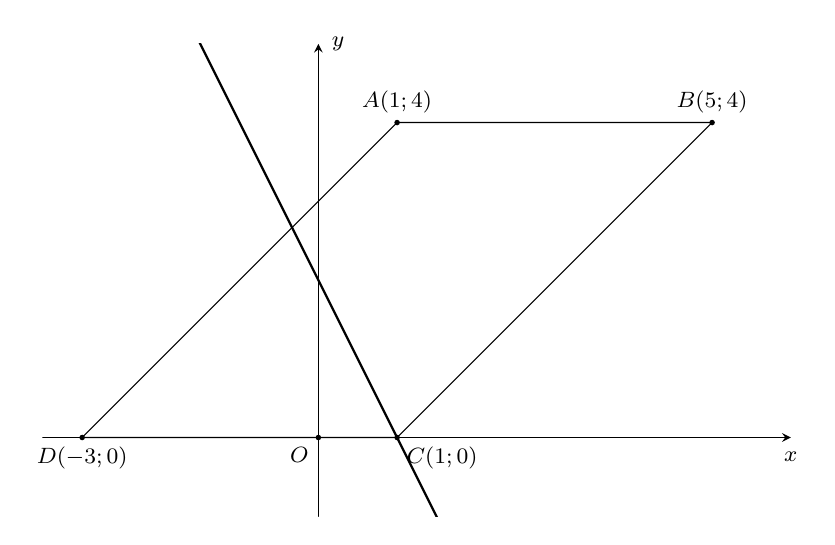
\begin{tikzpicture}[scale=1,>=stealth, font=\footnotesize, line join=round, line cap=round]	
	\tikzset{label style/.style={font=\footnotesize}}
	\def \xmin{-3.5}\def \xmax{6}\def \ymin{-1}\def \ymax{5} 
	\draw[->] (\xmin,0)--(\xmax,0) node[shift=(-90:0.25)] {$x$};
	\draw[->] (0,\ymin)--(0,\ymax) node[shift=(0:0.25)] {$y$};
	\fill[black] 
	(0,0)node [below left]{$O$} circle(1pt) 
	(1,0)node [below right]{$C(1;0)$} circle(1pt)
	(-3,0)node [below]{$D(-3;0)$} circle(1pt) 
	(1,4)node [above]{$A(1;4)$} circle(1pt) 
	(5,4)node [above]{$B(5;4)$} circle(1pt) 
	; 
	\draw (1,4)--(5,4)--(1,0)--(-3,0)--cycle;
	\begin{scope}
		\clip (\xmin,\ymin) rectangle (\xmax,\ymax); 
		\draw[thick,samples=200,domain=\xmin:\xmax,smooth,variable=\x] plot
		(\x,{-2*((\x))+2});
	\end{scope}
\end{tikzpicture}
\end{center}
Đa giác $ABCD$ giới hạn bởi miền $D\colon \heva{&y \geq 0 \\&y \leq 4 \\ &x-y+3 \geq 0 \\ &x-y-1 \leq 0.}$\\
Với mỗi $x \in \mathbb{Z}$ ta chọn số nguyên $y \in \mathbb{Z}$ nằm trong miền đa giác $ABCD$.\\
Ta mô tả không gian mẫu như sau
\begin{center}
	\begin{tabular}{|c|c|c|c|c|c|c|c|c|}
		\hline 
		$ (-3;0) $&$(-2;0) $&$(-1;0)$ &$(0;0)$ &$(1;0)$& & & &  \\
		\hline 
		&$ (-2;1) $&$ (-1;1) $ &$ (0;1) $ &$ (1;1) $&$ (2;1) $ & & & \\
		\hline 
		& &$ (-1;2) $ &$ (0;2) $ &$ (1;2) $& $ (2;2) $&$ (3;2) $ & & \\
		\hline 
		& & &$ (0;3) $ & $ (1;3) $&$ (2;3) $ &$ (3;3)  $&$ (4;3) $ & \\
		\hline 
		& & & & $ (1;4) $&$ (2;4) $ & $ (3;4) $&$ (4;4) $ &$(5;4)$ \\
		\hline
	\end{tabular}
\end{center}
Số phần tử của không gian mẫu $n(\Omega)=25$.\\
Đặt $Q$ là biến cố: \lq\lq  Chọn điểm $M$ có tọa độ nguyên nằm trong hoặc trên miền tứ giác mà có tọa độ nguyên thỏa mãn $2x+y>2$\rq\rq.\\
Ta có $n(Q)=15$.\\
Khi đó xác suất của biến cố $Q$ là $
p(Q)=\dfrac{n(Q)}{n(\Omega)}=\dfrac{15}{25}
$.
}
\end{ex}


\begin{ex}%[Đề thi thử môn Toán 12,THPT Phan Châu Trinh, Đà Nẵng]%[Anh Duy, 12EX-6-2223]%[2H2G2-2]%Câu 48
	Cho hình chóp $S.ABC$ có đáy $ABC$ là tam giác vuông tại $B$ với $BC=a$. Biết $S A=a \sqrt{2}$; hình chiếu vuông góc của $S$ lên mặt phẳng $(ABC)$ là trung điểm đoạn $AB$ và khoảng cách giữa hai đường thẳng $AC$ và $S B$ bằng $\dfrac{a \sqrt{6}}{3}$. Thể tích khối cầu ngoại tiếp hình chóp $S.ABC$ là
	\choice
	{\True $\dfrac{5 \sqrt{5}\pi a^3}{6}$}
	{$\dfrac{3 \sqrt{5}\pi a^3}{8}$}
	{$\dfrac{3 \sqrt{3}\pi a^3}{2}$}
	{$\dfrac{3 \sqrt{5}\pi a^3}{2}$}
	\loigiai{
		\begin{center}
			\begin{tikzpicture}[scale=0.7,>=stealth, font=\footnotesize, line join=round, line cap=round]	
				\def\r{3}
				\path
				(0,0) coordinate (B) 
				(-125:7) coordinate (A)
				(0:5) coordinate (C)
				($(A)!.5!(B)$) coordinate (H)
				($(H)+(90:6)$) coordinate (S)
				($(A)!.5!(C)$) coordinate (N)
				($(A)+(B)-(C)$) coordinate (x)
				($(B)!.6!(x)$) coordinate (t)
				(intersection of A--S and B--t) coordinate (B')
				($(B)!(H)!(B')$) coordinate (K)
				($(S)!.7!(K)$) coordinate (L)
				;
				\draw[dashed]
				(A)--(B)--(C)
				(S)--(B) (S)--(H)
				(B)--(B')
				(H)--(K)--(S)
				(H)--(L)
				(B)--(N)--(H)
				;
				\draw(A)--(S)--(C)--cycle
				(B')--(t) node[above]{$t$}
				(S)--(N)
				;
				\tkzMarkRightAngles(A,B,C H,K,B S,H,A K,L,H)
				\foreach \x/\g in
				{A/-90,B/90,C/0,S/90,H/-90,N/-90,K/-90,L/180}
				\fill[black](\x) circle (2pt)
				($(\x)+(\g:5mm)$) node{$\x$};
			\end{tikzpicture}
		\end{center}
Gọi $H$ là trung điểm của $AB \Rightarrow S H \perp AB$. Gọi $N$ là trung điểm của $A C$.\\
Trong mặt phẳng $(ABC)$ kẻ $Bt \parallel  AC, HK \perp Bt, K \in Bt$.\\
Trong mặt phẳng $(HSK)$ kẻ $HL \perp SK, L \in SK$, khi đó ta có
$$
 \mathrm{d}(H,(S, Bt))=HL=\dfrac{1}{2}\mathrm{d}(A,(S,Bt))=\dfrac{1}{2}\mathrm{d}(AC, SB)=\dfrac{a \sqrt{6}}{6}.
$$
Đặt $AB=2x$, $(x>0)$.\\
Ta có tam giác $SHA$ vuông tại $H$ nên $SH^2=SA^2-AH^2=2 a^2-x^2$.\\
Tam giác $SHK$ vuông tại $H$ nên 
$$
\begin{aligned}
	& \Rightarrow \dfrac{1}{HL^2}=\dfrac{1}{HK^2}+\dfrac{1}{SH^2}=\dfrac{4}{\mathrm{d}^2(B, AC)}+\dfrac{1}{SH^2}=4\left(\dfrac{1}{AB^2}+\dfrac{1}{BC^2}\right)+\dfrac{1}{SH^2}\\
	& \Rightarrow \dfrac{1}{x^2}+\dfrac{1}{2 a^2-x^2}=\dfrac{2}{a^2}\Rightarrow x=a \Rightarrow S H=a.
\end{aligned}
$$
Do $SH=a=\dfrac{1}{2}AB \Rightarrow \triangle SAB$ vuông cân tại $S \Rightarrow HA=HB=HS=a$.\\
Ta có $HN \perp(SAB) \Rightarrow NA=NB=NS$. \hfill $(1)$\\
Do tam giác $ABC$ vuông tại $B$, $N$ là trung điểm của $AC \Rightarrow NA=NB=NC$. \hfill $(2)$\\
Từ $(1)$, $(2)$ suy ra $ N$ là tâm mặt cầu ngoại tiếp hình chóp $S.ABC \Rightarrow R=NC=\dfrac{1}{2}AC=\dfrac{a \sqrt{5}}{2}$.\\
Thể tích khối cầu ngoại tiếp hình chóp $S.ABC$ là $V=\dfrac{4}{3}\pi R^3=\dfrac{5 \sqrt{5}a^3 \pi}{6}$.	
}
\end{ex}

\begin{ex}%[Đề thi thử môn Toán 12,THPT Phan Châu Trinh, Đà Nẵng]%[Anh Duy, 12EX-6-2223]%[2D2G6-5]%Câu 49
	Có bao nhiêu cặp số nguyên dương $(x; y)$ và $x \leq 93$ thoả mãn điều kiện $$4\left(2^{3y}+6 y\right) \leq x+8 \log _2(x+7)-9?$$
	\choice
	{$106$}
	{\True $69$}
	{$2$}
	{$92$}
	\loigiai{
Ta có
$$
4\left(2^{3y}+6 y\right) \leq x+8 \log _2(x+7)-9 \Leftrightarrow 2^{3y+2}+8(3y+2) \leq 2^{\log _2(x+7)}+8 \log _2(x+7).\quad (*)
$$
Xét hàm số $f(t)=2^t+8 t$, ta có $f'(t)=2^t \ln 2+8>0, \forall t$ nên hàm số $f(t)$ đồng biến.\\
Khi đó 
\begin{eqnarray*}
(*) &\Leftrightarrow& f(3y+2) \leq f\left(\log _2(x+7)\right)\\
&\Leftrightarrow& 3y+2 \leq \log _2(x+7)\\
& \Leftrightarrow& y \leq \dfrac{\log _2(x+7)-2}{3}.
\end{eqnarray*}
Vì $y \in \mathbb{Z}^{+}$ nên $\dfrac{\log _2(x+7)-2}{3}\geq 1 \Leftrightarrow x \geq 25$.\\
Mặt khác $x \leq 93$ suy ra $$y \leq \dfrac{\log _2(x+7)-2}{3}\leq \dfrac{\log _2(93+7)-2}{3}\approx 1{,}548.$$
Do đó ứng với mỗi $25 \leq x \leq 93$ luôn xác định được duy nhất giá trị $y=1$.\\
Vậy có $69$ cặp số nguyên dương $(x; y)$.
}
\end{ex}

\Closesolutionfile{ans}
\indapan{10}{ans/ans-2-TT-1-THPTPhanChauTrinh-DaNang-23}